\documentclass[a4paper, 12pt]{article}

\usepackage[table,xcdraw]{xcolor}
\usepackage{enumerate}
\usepackage{enumitem}
\usepackage{graphicx}
\usepackage[T5]{fontenc}
\usepackage[utf8]{inputenc}
\usepackage[margin = 2cm]{geometry}
\usepackage{amsfonts, amsmath, amssymb}
\usepackage[none]{hyphenat}
\usepackage{fancyhdr}
\usepackage{float}
\usepackage{hyperref}
\usepackage{physics}
\usepackage{caption}
\usepackage{subcaption}
\usepackage[nottoc, notlot, notlof]{tocbibind}

\usepackage{mathtools}
\DeclarePairedDelimiter\ceil{\lceil}{\rceil}
\DeclarePairedDelimiter\floor{\lfloor}{\rfloor}
% for code section
\usepackage{listings}

% for sub-figure
\usepackage{subcaption}
% \usepackage{rotating}
% \usepackage{tikz}

\captionsetup[table]{skip=5pt}
\pagestyle{fancy}
\fancyhead[L]{Trường Đại học Khoa học Tự nhiên - ĐHQG TP.HCM}
\fancyhead[R]{Nhóm 9}

% Paragraph format
\setlength{\parindent}{0em}
\setlength{\parskip}{1em}

\begin{document}

\begin{titlepage}
    \begin{center}
        %\vspace*{1cm}
        \Large\textbf{Đại học Quốc gia TP. HCM\\Trường Đại học Khoa học Tự nhiên\\Bộ Môn Khoa học Máy tính}\\

        \vspace*{1cm}
        \begin{figure}[H]
            \begin{center}
                
\includegraphics[scale=0.2]{images/hcmus-logo}
            \end{center}
        \end{figure}
        \line(1,0){450}\\[4mm]
        \LARGE\textbf{\MakeUppercase{Báo cáo Seminar Cuối kì\\ Face Recognition}}\\[3mm]
        \Large{Nhận Dạng (CSC14006)}\\[3mm]
        \Large{Nhóm 9}
        \line(1,0){430}\\

        \vfill
        TP Hồ Chí Minh, ngày 01/06/2021
    \end{center}
\end{titlepage}

\tableofcontents
\thispagestyle{empty}
\clearpage

\section{Thông tin nhóm}
    \begin{table}[H]
        \centering
        \begin{tabular}{|c|c|l|c|c|}
        \hline
        STT & MSSV     & \multicolumn{1}{c|}{Họ tên} & Email\\ \hline
        1   & 18120078 & Ngô Phù Hữu Đại Sơn         & 18120078@student.hcmus.edu.vn\\ \hline
        2   & 18120533 & Dương Đoàn Bảo Sơn          & 18120533@student.hcmus.edu.vn\\ \hline
        3   & 18120164 & Lê Minh Đức                 & 18120164@student.hcmus.edu.vn\\ \hline
        \end{tabular}
        \caption{Bảng danh sách thành viên nhóm}
    \end{table}

\section{Phân công các thành viên trong nhóm}

    \begin{table}[H]
        \centering
        \begin{tabular}{|c|l|l|c|}
        \hline
        STT & \multicolumn{1}{c|}{Họ tên} & \multicolumn{1}{c|}{Công việc tham gia}  & Hoàn thành (\%) \\ \hline
        1   & Ngô Phù Hữu Đại Sơn         & CNNS, ResNet và ArcFace loss             & 100/100 \\ \hline
        2   & Dương Đoàn Bảo Sơn          & Databases                                & 100/100 \\ \hline
        5   & Lê Minh Đức                 & Các kỹ thuật cơ bản nhận dạng            & 100/100 \\ \hline
        \end{tabular}
        \caption{Bảng phân tích tỷ lệ hoàn thành công việc}
    \end{table}
\clearpage

\section{Lý thuyết}
\subsection{Kiến thức về Local Binary Patterns (LBP)}

\subsubsection*{Đặc trưng ảnh cục bộ (Local Image Texture)}
Dấu của hiệu giá trị các pixel xung quanh so với điểm ảnh ở tâm sẽ bất biến với phép chiếu sáng.

\begin{equation}
	T \sim t(s(g_0-g_c), s(g_1-g_c),\ldots,s(g_{P-1} - g_c))
\end{equation}

Có 2 kiểu đặc trưng cục bộ:
\begin{itemize}
	\item \textit{Vuông (Square Neighborhood):} Các điểm trên vùng đặc trưng cục bộ xếp thành hình vuông (đi theo chiều vòng tròn lượng giác), điểm $g_0$ cách điểm $g_c$ một khoảng R (bán kính) pixel. 
	\item \textit{Tròn (Circular Neighborhood):} Các điểm trên vùng đặc trưng cục bộ xếp thành hình tròn (đi theo chiều vòng tròn lượng giác), điểm $g_0$ cách điểm $g_c$ một khoảng R (bán kính) pixel. Do xếp theo hình tròn nên sẽ có một số điểm phải sử dụng phép nội suy để tính. Trong các nội dung bên dưới, xin sử dụng đặc trưng tròn để bàn.
\end{itemize}
\begin{figure}[H]
	\begin{center}
		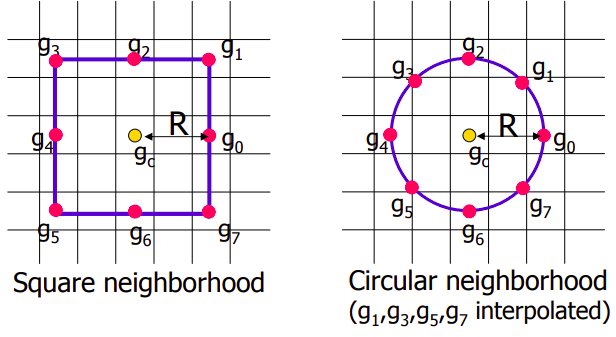
\includegraphics[scale=0.6]{images/theo1/local_image_texture}
		\caption{Đặc trưng vuông bên trái, đặc trưng tròn bên phải}
	\end{center}
\end{figure}
\pagebreak

\subsubsection{LBP\textsubscript{P,R} (1996)}

$LBP_{P,R}$ xác định giá trị tại điểm ảnh $g_c$ bằng đặc trưng ảnh cục bộ của các điểm xung quanh điểm ảnh đó qua công thức:
\begin{equation}
	LBP_{P,R} = \sum^{P-1}_{p=0}{s(g_p-g_c)\times 2^p}
\end{equation}
Trong đó:
\begin{itemize}
	\item \textit{P(Point)} là số lượng điểm trong vùng đặc trưng cục bộ, mỗi điểm cách nhau một khoảng $\frac{2\pi}{P}$ rad.
	\item \textit{R(Radius)} là bán kính của vùng đặc trưng cục bộ.
	\item $g_c$ là điểm cần tính giá trị $LBP_{P,R}$ (Tâm của hình vuông hay hình tròn).
	\item $g_p$ là điểm thứ p trên vùng đặc trưng cục bộ.
	\item \textit{s (sign function)} là hàm dấu:
		\begin{equation}
			s(x) = \begin{cases}
				1, & x \geq 0\\
				0, & x < 0
			\end{cases}
		\end{equation}
\end{itemize}

\textit{Ví dụ}: Giá trị của $LBP_{8,1}$ của điểm ảnh ở giữa (hình 2) được tính như sau:
$$
	LBP_{8,1} = \sum^{7}_{p=0}{s(g_p-76)\times 2^p} = 1 + 2 +2^3 + 2^5 + 2^6 = 107
$$

\begin{figure}[H]
	\begin{center}
		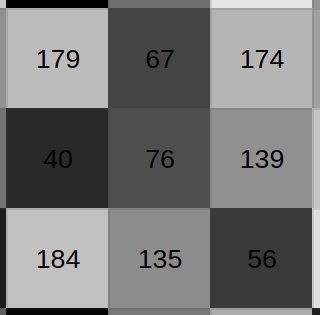
\includegraphics[scale=0.5]{images/theo1/LBP_exam1}
		\caption{Ví dụ $LBP_{P,R}$}
	\end{center}
\end{figure}
\pagebreak

\underline{Ưu điểm}
\begin{itemize}
	\item Bất biến với phép chiếu sáng. Giúp giảm FRR (False Reject Rate) cho các ảnh được chụp ở các điều kiện sáng tối khác nhau. \\
	\textit{Ví dụ}: Độ sáng tăng lên nhưng $LBP_{8,1}$ không thay đổi (Hình 3).
	$$
		LBP_{8,1} = \sum^{7}_{p=0}{s(g_p-76)\times 2^p} = 1 + 2 +2^3 + 2^5 + 2^6 = 107
	$$
	\begin{figure}[H]
		\begin{center}
			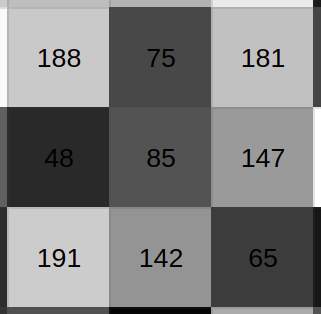
\includegraphics[scale=0.5]{images/theo1/LBP_exam2}
			\caption{$LPB_{P,R}$ bất biến phép chiếu sáng}
		\end{center}
	\end{figure}
	\item Không cần phải so sánh 2 vector đặc trưng (Công thức 1).
	\item Tính toán đơn giản.
\end{itemize}
\underline{Nhược điểm}
\begin{itemize}
	\item Không bất biến với phép xoay.\\
	\textit{Ví dụ:} khi xoay hình 90 độ theo ngược chiều kim đồng hồ, ta sẽ có giá trị $LBP_{8,1}$ thay đổi (Hình 3).
	$$
		LBP_{8,1} = \sum^{7}_{p=0}{s(g_p-76)\times 2^p} = 1 + 2^2 + 2^3 + 2^5 + 2^7 = 173
	$$
	\begin{figure}[H]
		\begin{center}
			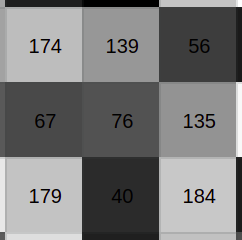
\includegraphics[scale=0.6]{images/theo1/LBP_exam3}
			\caption{$LBP_{P,R}$ không bất biến với phép xoay}
		\end{center}
	\end{figure}
\end{itemize}


\subsubsection{LBP\textsubscript{P,R}\textsuperscript{ri} (2000)}
Khắc phục được nhược điểm của $LBP_{P,R}$, $LBP_{P,R}^{\text{  }ri}$ bất biến với cả phép quay và phép chiếu sáng bằng cách sử dụng giá trị nhỏ nhất để đại diện cho tất cả các ảnh xoay (ảnh được xoay theo chiều đường tròn lượng giác với một góc không đổi).

\begin{equation}
	LBP_{8,1}^{\text{  }ri} = \min_{i=0 \to P-1}{ROR(LBP_{8,1}, i)}
\end{equation}
\textit{Trong đó:}
\begin{itemize}
	\item \textit{ROR(x, i)} là phép xoay bit sang phải của x theo vòng tròn i lần. Tương ứng với việc xoay tập hợp các hàng xóm theo chiều kim đồng hồ.
\end{itemize}

\textit{Ví dụ}: Giá trị của $LBP_{8,1}^{\text{  }ri}$ của điểm ảnh ở giữa (hình 2) được tính như sau:
\begin{align*}
	01101011_2 &= 107\\
	10110101_2 &= 181\\
	11011010_2 &= 218\\
	01101101_2 &= 109\\
	10110110_2 &= 182\\
	01011011_2 &= 91  \text{   (Nhỏ nhất)}\\
	10101101_2 &= 173\\
	11010110_2 &= 214\\
\end{align*}
$$
	\Longrightarrow LBP_{8,1}^{\text{  }ri} = \min_{i=0 \to P-1}{ROR(LBP_{8,1}, i)} = 91
$$
\subsubsection{LBP\textsubscript{P,R}\textsuperscript{riu2} (2002)}

Đặc trưng của $LBP_{P,R}^{\text{  }riu2}$ khắc phục được nhược điểm của $LBP_{P,R}^{\text{  }ri}$ đó là:
\begin{itemize}
	\item Tính toán nhanh và đơn giản. Với mỗi điểm ảnh, chỉ cần tính một giá trị.
	\item Sử dụng các \textit{Uniform Patterns} để  giảm các trường hợp phép xoay không mang lại nhiều ý nghĩa, do mỗi lần xoay cho các giá trị khác nhau làm không thể hiện đươc đặc thù của điểm ảnh.
\end{itemize}
\pagebreak

\textbf{Uniform Patterns:} Một mẫu nhị phân được gọi là đồng dạng khi xét chuỗi bit xoay vòng thì có nhiều nhất là 2 lần thay đổi (transitions) từ giá trị bit 0 sang 1 hoặc từ giá trị bit 1 sang 0. 

\textit{Ví dụ: }Với hàng đầu tiên là 9 mẫu \textit{Uniform}. Còn lại là các mẫu \textit{Non-Uniform}. Các mẫu Non-Uniform không mang lại nhiều ý nghĩa trong nhận dạng.
\begin{figure}[H]
	\begin{center}
		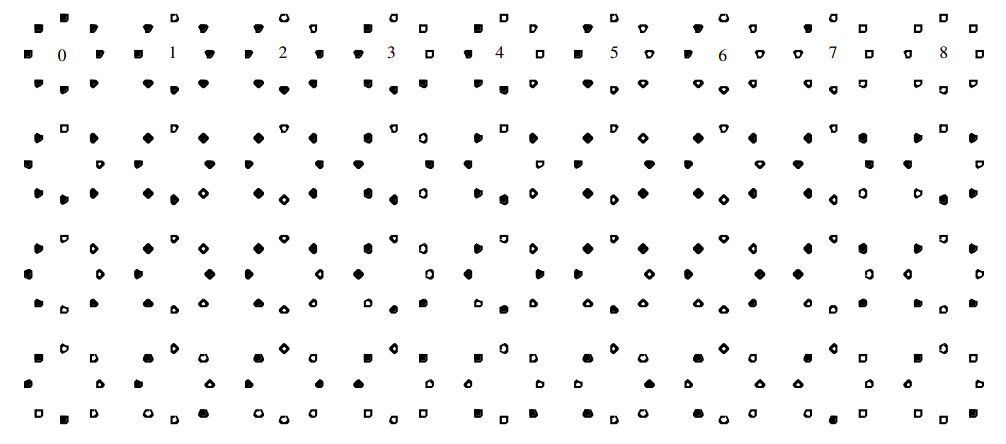
\includegraphics[scale=0.4]{images/theo1/uniform_exam}
		\caption{36 mẫu nhị phân khác nhau của $LPB_{8,R}^{\text{  ri}}$}
	\end{center}
\end{figure}

\begin{equation}
	LBP_{P,R}^{\text{  }riu2}=\begin{cases}
		\sum_{p=0}^{P-1}{s(g_p-g_c)}  & U(LBP_{P,R}\leq 2)\\
		P + 1 & U(LBP_{P,R}) > 2
	\end{cases}
\end{equation}
\textit{Trong đó:}
$$
	U(LBP_{P,R})=\left\lvert s(g_{P-1} - g_c)-s(g_0-g_c)\right\rvert + \sum_{p=1}^{P-1}{\left\lvert s(g_p - g_c)-s(g_{p-1}-g_c)\right\rvert}
$$

\textit{Chú thích:} 
\begin{itemize}
	\item Hàm \textit{U} thể hiện số lần chuyển từ bit 0 sang bit 1 và ngược lại của các điểm trên đường tròn.
	\item \textit{LBP\textsubscript{P,R}\textsuperscript{riu2}} là số lượng bit 1 trên đường tròn nếu mẫu đang xét Uniform. Ngược lại, bằng P + 1 nếu mẫu không Uniform.
\end{itemize}
\pagebreak

\textit{Ví dụ:}
\begin{itemize}
	\item Uniform Pattern 
	$$
		LBP_{P,R}^{\text{  }riu2} = 5
	$$
	\begin{figure}[H]
		\begin{center}
			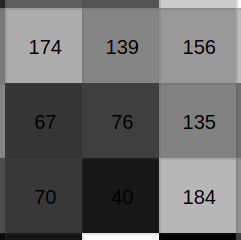
\includegraphics[scale=0.65]{images/theo1/LBP_exam4}
			\caption{Uniform Pattern}
		\end{center}
	\end{figure}
	\item Non-Uniform Pattern
	$$
		LBP_{P,R}^{\text{  }riu2} = 9
	$$
	\begin{figure}[H]
		\begin{center}
			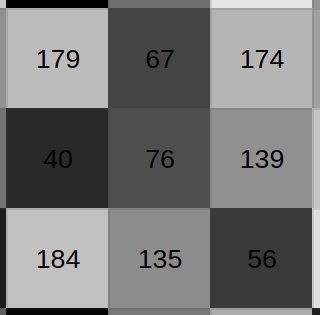
\includegraphics[scale=0.5]{images/theo1/LBP_exam1}
			\caption{Non-Uniform Pattern}
		\end{center}
	\end{figure}
\end{itemize}

\subsubsection{Adjacent Evaluation LBP (AELBP)}
\begin{equation}
	AELBP_{P,R}=\sum_{p=0}^{P-1}{s(a_p-g_c)\times 2^p}
\end{equation}
\textit{Trong đó:}
\begin{itemize}
	\item $a_p$ được tính bằng cách xem $g_p$ là tâm của một block(adjacent evaluation window) có kích thước W$\times$W (W cho trước). Sau đó, $a_p$ là giá trị trung bình của các điểm ảnh trong block đó (Không bao gồm $g_p$). Lưu lý W=1 thì AELBP có giá trị bằng với LBP.
\end{itemize}

\textit{Ví dụ:} Trong ví dụ dưới, ta chọn điểm $g_0$ tại góc trái trên, chiều quay ngược chiều lượng giác và W = 3. Song việc tính toán sẽ tương tự khi $g_0$ về góc lượng giác và chiều lượng giác như các phần trình bày trước.
$$
	AELBP_{P,R}=\sum_{p=0}^{P-1}{s(a_p-118)\times 2^p}=255
$$
\begin{figure}[H]
	\begin{center}
		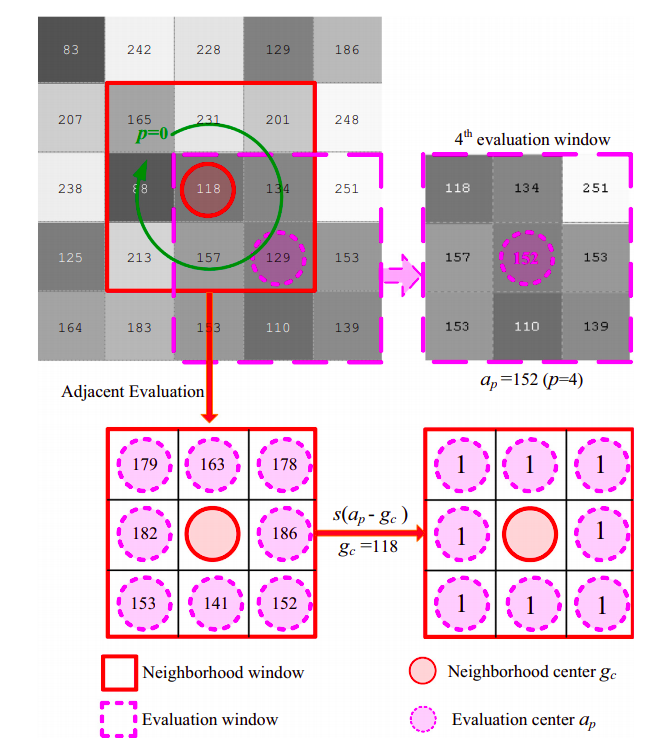
\includegraphics[scale=0.5]{images/theo1/AELBP}
		\caption{Ví dụ AELBP}
	\end{center}
\end{figure}

\underline{Ưu điểm}
\begin{itemize}
	\item AELBP có thể nhận dạng tốt các ảnh có nhiều noise, bằng cách sử dụng giá trị trung bình của lân cận với các điểm $g_p$. Trong khi LBP thông thường lại rất nhạy cảm với noise.
\end{itemize}
\underline{Nhược điểm}
\begin{itemize}
	\item Tính toán phức tạp hơn so với LBP thông thường.
\end{itemize}
\subsection{Kiến thức PCA (Principal Component Analysis) và (LDA) Linear Discriminant Analysis }

\subsubsection{PCA}
Giả sử ta có: $\langle x_1, x_2, \ldots, x_M \rangle_{N \times 1}$. Quá trình thực hiện giảm chiều tập dữ liệu trên bằng PCA được thực hiện qua các bước sau:
\begin{itemize}
	\item \textbf{Bước 1: }Tính các giá trị trung bình của các biến
	\begin{equation}
		\bar{x} = \frac{1}{M}\sum_{i=1}^{M}{x_i}
	\end{equation}
	\item \textbf{Bước 2: }Dời gốc tọa độ về điểm trung bình trong không gian dữ liệu.
	\begin{equation}
		\Phi_i = x_i - \bar{x}
	\end{equation}
	\item \textbf{Bước 3: }Tính ma trận hiệp phương sai:
	\begin{equation}
		C = \frac{1}{M}\sum_{m=1}^{M}{\Phi_m \Phi_m^T}
	\end{equation}
	\item \textbf{Bước 4: }Tính các trị riêng của C
	\begin{equation}
		\lambda_1 > \lambda_2 > \cdots > \lambda_N
	\end{equation}
	\item \textbf{Bước 5: }Tính các vector riêng tương ứng
	\begin{equation}
		u_1, u_2,\ldots,u_N
	\end{equation}
	\item \textbf{Bước 6: }Giữ lại K vector riêng có trị riêng tương ứng lớn nhất. Do ma trận hiệp phương sai đối xứng, nên các vector riêng đôi một song song nhau và tạo thành một hệ cơ sở. Ma trận chuyển không gian U được hình thành như sau:
	\begin{equation}
		U = \left[u_1, u_2, \ldots, u_K\right]
	\end{equation}
	\item \textbf{Bước 7: }Các điểm dữ liệu được chuyển qua không gian mới (có số chiều K << N) theo công thức:
	\begin{equation}
		b = U^T\left(x - \bar{x}\right)
	\end{equation}
\end{itemize}
\pagebreak

\textit{Ví dụ minh họa:}
Có các điểm sau (2.5, 2.4), (0.5, 0.7), (2.2, 2.9), (1.9, 2.2), (3.1,3.0), (2.3, 2.7), (2, 1.6), (1, 1.1), (1.5, 1.6), (1.1, 0.9). Sử dụng PCA để giảm chúng về 1 chiều.
\begin{itemize}
    \item \textbf{Bước 1:} Tính trung bình, chuẩn hóa.
    \begin{figure}[H]
        \begin{center}
            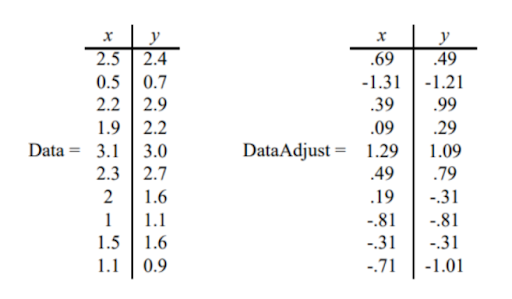
\includegraphics[scale=0.7]{images/theo2/PCA-cal-1}
            \caption{Tính trung bình, chuẩn hóa}
        \end{center}
    \end{figure}

    \item \textbf{Bước 2:} Ma trận hiệp phương sai.
    \begin{figure}[H]
        \begin{center}
            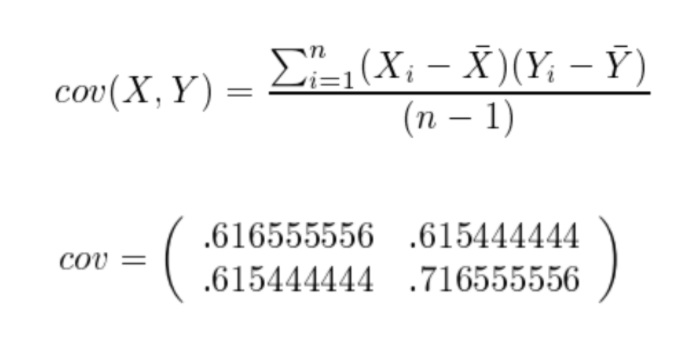
\includegraphics[scale=0.4]{images/theo2/PCA-cal-2}
            \caption{Ma trận hiệp phương sai}
        \end{center}
    \end{figure}

    \item \textbf{Bước 3:} Tính vector riêng và giá trị riêng cho ma trận hiệp phương sai.
    \begin{figure}[H]
        \begin{center}
            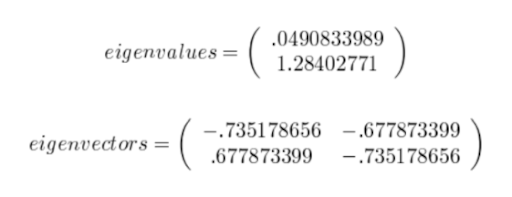
\includegraphics[scale=0.5]{images/theo2/PCA-cal-3}
            \caption{Ma trận hiệp phương sai}
        \end{center}
    \end{figure}
    
    \item \textbf{Bước 4:} Biến đổi dữ liệu:
    \begin{figure}[H]
        \begin{center}
            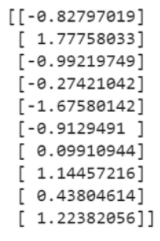
\includegraphics[scale=0.5]{images/theo2/PCA-cal-4}
            \caption{Dữ liệu sao khi biến đổi}
        \end{center}
    \end{figure}
\end{itemize}

\subsubsection{LDA}

\begin{itemize}
    \item \textbf{Bước 1:} Tính ma trận phân tán giữa các nhóm.
    \begin{equation}
        S_B=\sum_{i=1}^{C}{c_i(\mu_i - \mu)(\mu_i-\mu)^T}
    \end{equation}
    \subitem $\mu_i$ là giá trị trung bình của từng lớp. 
    \subitem $\mu$ là giá trị trung bình của tất cả dữ liệu. 

    \item \textbf{Bước 2:} Tính ma trận phân tán tích lũy ứng với từng nhóm.
    \begin{equation}
        S_W=\sum_{j=1}^{C}{\sum_{i=1}^{n_j}{(x_{ij}-\mu_j)(x_{ij}-\mu_j)^T}}
    \end{equation}

    \item \textbf{Bước 3:} Xây dựng hàm tiêu chí tách lớp.
    \begin{equation}
        W = S_W^{-1}S_B
    \end{equation}

	\item \textbf{Bước 4:} Tính các vector riêng (chọn ra tối đa C - 1 vector riêng có giá trị riêng tương ứng lớn nhất) của W. Từ đó hình thành ma trận đổi cơ sở:
	\begin{equation}
		U = \left[w_1, w_2, \ldots, w_{C-1}\right]
	\end{equation}

	\item \textbf{Bước 5:} Chuyển các điểm dữ liệu sang không gian mới
	\begin{equation}
		y = U^T(x - \mu)
	\end{equation}
\end{itemize}
\pagebreak

\textit{Ví dụ:} Cho tập dữ liệu:
$$
X = \left( \begin{array}{cc}
	4 & 1 \\
	2 & 4 \\
	2 & 3 \\
	3 & 6 \\
	4 & 4 \\
	9 & 10 \\
	6 & 8 \\
	9 & 5 \\
	8 & 7 \\
	10 & 8 \\

\end{array} \right)
%
y = \left( \begin{array}{c}
	1 \\
	1 \\
	1 \\
	1 \\
	1 \\
	2 \\
	2 \\
	2 \\
	2 \\
	2 \\
\end{array} \right)
$$

\textit{Ta có:} 
$$
\mu_1 = \left( \begin{array}{c}
	3.0 \\
	3.6
\end{array} \right)
%
\mu_2 = \left( \begin{array}{c}
	8.4 \\
	7.6	
\end{array} \right)
\mu = \left( \begin{array}{c}
	5.7 \\
	5.6	
\end{array} \right)
$$

\begin{itemize}
	\item \textbf{Bước 1:} Tính $S_B$
	$$
		S_B = \left( \begin{array}{cc}
			29.16 & 21.6\\
			21.6 & 16.0
		\end{array}\right)
	$$
	\item \textbf{Bước 2:} Tính $S_W$
	$$
		S_W = \left( \begin{array}{cc}
			2.64 & -0.44\\
			-0.44 & 5.28
		\end{array}\right)
	$$
	\item \textbf{Bước 3:} Tìm ma trận chuyển không gian, bước này tượng tự với các bước từ bước 3 trở về sau của PCA nhưng thay ma trận C bằng ma trận $W = S_W^{-1}S_B$
	$$
		\lambda = 15.65 
		\Longrightarrow w = \left( \begin{array}{c}
			0.91\\
			0.39
		\end{array}\right)
	$$
	\item \textbf{Bước 4:} Chuyển các điểm dữ liệu về không gian mới ($b = w^Tx$)
	$$
		\left( \begin{array}{c}
			4.03 \\
			3.38 \\
			2.99 \\
			5.07 \\
			5.2 \\
			12.09 \\
			8.58 \\
			10.14 \\
			10.01 \\
			12.22 \\
		\end{array} \right)
	$$
\end{itemize}
\pagebreak

\subsubsection{Sự khác biệt giữa PCA và LDA}
\begin{itemize}
	\item PCA giảm chiều dữ liệu không quan tâm đến lớp của dữ liệu đó (Unsupervised Learning). Trong khi LDA lại quanh tâm đến lớp của các điểm dữ liệu (Supervised Learning).
	\item PCA giảm chiều xuống một giá trị K nhỏ hơn số thuộc tính của dữ liệu. Trong khi LDA chỉ có thể  giảm số chiều sao cho số chiều giảm xuống phải nhỏ hơn số lớp trong tập dữ liệu.
	\item LDA sẽ cho kết quả tốt hơn trên tập huấn luyện vì có quan tâm đến nhãn.
	\item LDA dễ gặp các trường hợp suy biến khi chiều ban đầu của dữ liệu rất lớn như số lượng điểm dữ liệu trong tập lại quá nhỏ. Ví như các dữ liệu ảnh.
\end{itemize}
\begin{figure}[H]
	\begin{center}
		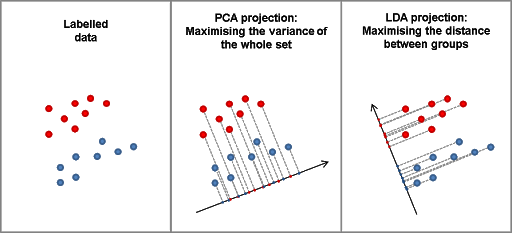
\includegraphics[scale = 0.5]{images/theo2/LDA-PCA-cmp}
		\caption{So sánh LDA và PCA}
	\end{center}
\end{figure}
\subsection{Kiến thức về Support Vector Machines (SVM)}
\begin{itemize}
    \item Chọn hàm \textit{Kernel}.
	\item Chọn giá trị điều khiển biến cho dữ liệu huấn luyện C.
	\item Bài toán tối ưu bậc hai để tìm tham số cho vector hỗ trợ.
	\item Xây dựng hàm tách lớp từ các vector hỗ trợ.
\end{itemize}

\subsubsection{Ví dụ minh họa SVM}
\begin{itemize}
    \item Đối với dữ liệu tuyến tính:
    \begin{figure}[H]
        \begin{center}
            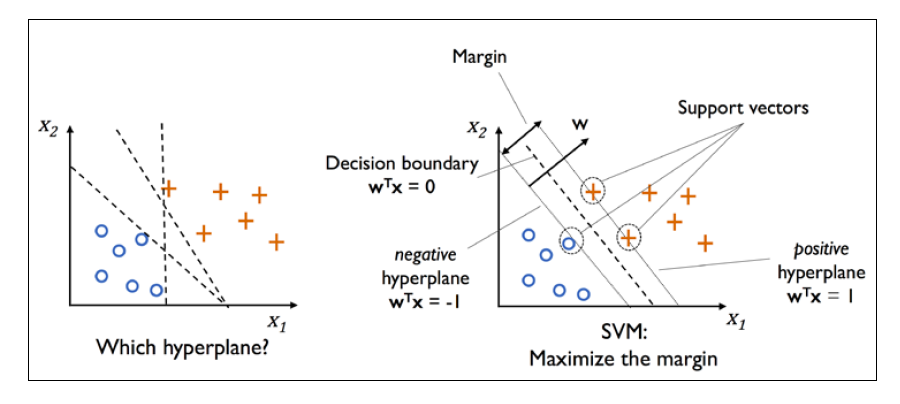
\includegraphics[scale=0.3]{images/theo3/SVM-ex-2}
            \caption{SVM với dữ liệu tuyến tính}
        \end{center}
    \end{figure}

    \item Đối với dữ liệu phi tuyến ta không thể chia trực tiếp bằng các đường thẳng, ta cần phải sử dụng hàm \textit{Kernel} để ánh xạ dữ liệu đó vào không gian nhiều chiều hơn:
    \begin{figure}[H]
        \begin{center}
            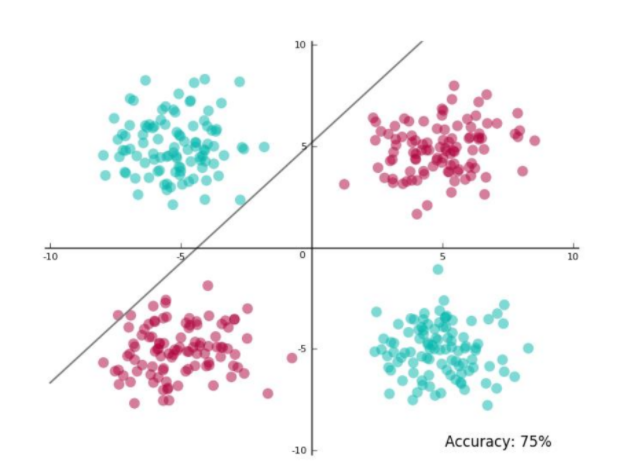
\includegraphics[scale=0.3]{images/theo3/SVM-kernel-1}
            \caption{SVM với dữ liệu phi tuyến}
        \end{center}
    \end{figure}
    \subitem Ta sử dụng hàm \textit{Kernel} để ánh xạ tập dữ liệu 2 chiều trên thành dữ liệu 3 chiều từ đó dễ dàng tìm ra siêu phẳng để phân lớp hơn.
    \begin{figure}[H]
        \begin{center}
            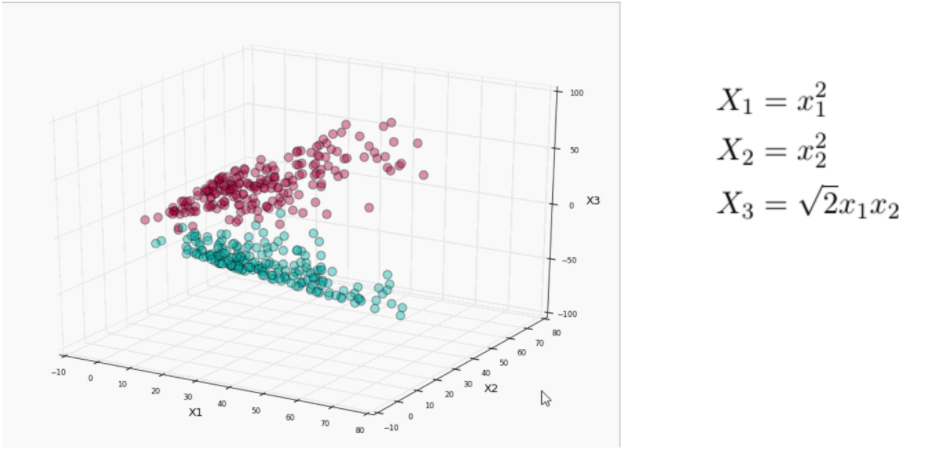
\includegraphics[scale=0.3]{images/theo3/SVM-kernel-2}
            \caption{Tăng chiều dữ liệu bằng các hàm kernel}
        \end{center}
    \end{figure}
\end{itemize}

\subsubsection{Một số hàm kernel thông dụng}
\begin{itemize}
    \item Hàm tuyến tính: $K(x_i, x_j) = x_i^Tx_j$.
    \item Hàm đa thức: $K(x_i, x\_j) = (1 + x_i^Tx_j)^p$
    \item Gaussian: $K(x_i, x_j) = e^{-\frac{\|x_i-x_j\|^2}{2\sigma^2}}$.
    \item Sigmoid: $K(x_i, x_j) = tanh(\beta_0x_i^Tx_j + \beta_1)$
\end{itemize}

\subsubsection{Phân biệt chiến lược one vs all và one vs one}
\begin{itemize}
    \item \textbf{One vs One: }Xây dựng rất nhiều bộ binary classifiers cho từng cặp classes. Bộ thứ nhất phân biệt class 1 và class 2, bộ thứ hai phân biệt class 1 và class 3, … Khi có một dữ liệu mới vào, đưa nó vào toàn bộ các bộ binary classifiers trên. Kết quả cuối cùng có thể được xác định bằng cách xem class nào mà điểm dữ liệu đó được phân vào nhiều nhất (major voting). Như vậy, nếu có C classes thì tổng số binary classifiers phải dùng là n(n – 1)/2. Đây là một con số lớn, cách làm này không lợi về tính toán.
    \item \textbf{One vs All: }Nếu có C classes thì ta sẽ xây dựng C classifiers, mỗi classifier tương ứng với một class. Classifier thứ nhất giúp phân biệt class 1 vs not class 1 , tức xem một điểm có thuộc class 1 hay không, hoặc xác suất để một điểm rơi vào class 1 là bao nhiêu. Tương tự như thế, classifier thứ hai sẽ phân biệt class 2 vs not class 2, … Kết quả cuối cùng có thể được xác định bằng cách xác định class mà một điểm rơi vào với xác suất cao nhất.
\end{itemize}
\subsection{Kiến thức về mạng nơron cơ bản (ANN)}
\subsubsection{Cấu trúc mạng đề nghị}
\textit{Gồm 3 tầng:}
\begin{enumerate}
	\item tầng nhập ảnh
	\item tầng cơ sở gồm 2 bộ phân lớp
	\begin{enumerate}
		\item Bộ phân lớp \textit{nam} hay \textit{nữ}: Bộ phân lớp được huấn luyện với số lượng ảnh \textit{nam} là 5 và số lượng ảnh \textit{nữ} là 8, giúp cho việc huấn luyện bộ phân lớp tốt hơn.
		\item Bộ phân lớp \textit{tóc dài} hay \textit{tóc ngắn}: Bộ phân lớp được huận luyện với số lượng ảnh \textit{tóc dài} là 5 và số lượng ảnh \textit{tóc ngắn} là 8, nhờ vậy cũng giúp cho bộ phân lớp tốt hơn.
	\end{enumerate}
	\item tầng xuất gồm 4 bộ phân lớp: nhờ các bộ phân lớp ở tầng 2 đã được huấn luyện tốt, các bộ phân lớp ở tầng 3 sẽ chỉ cần ít dữ liệu thậm chí không cần dữ liệu để huấn luyện. Từ đó tránh được các lỗi phân loại sai.
	\begin{enumerate}
		\item Bộ phân lớp có phải \textit{nữ tóc dài}
		\item Bộ phân lớp có phải \textit{nam tóc dài}
		\item Bộ phân lớp có phải \textit{nữ tóc ngắn}
		\item Bộ phân lớp có phải \textit{nam tóc ngắn}
	\end{enumerate}
\end{enumerate}

\subsubsection{Tính hiệu quả của cấu trúc đề nghị}
Nhờ sử dụng thêm một tầng cơ sở chứa 2 bộ phân lớp có phân bố dữ liệu không lệch quá nhiều, nên kết quả của 2 bộ phân lớp trên khá tốt. Nhờ vào đó mà ở tâng 3 chỉ cần tổng hợp kết quả của tầng cơ sở mà không cần huấn luyện. Từ đó giải quyết được vấn đề dữ liệu ở tầng phân lớp ít.
\pagebreak
\subsection{Kiến thức về mạng nơron sâu (DNN)}
\subsubsection{mạng nơron sâu thường cho kết quả tốt hơn mạng nơron rộng với cùng số lượng nơron.}

Đối với mạng nơron có N nút, mạng học sâu có số tổ hợp các đường đi nhiều hơn rất nhiều so với mạng học rộng chỉ có một lớp. Nhờ đó các giá trị của hàm xấp xỉ sẽ gần đúng với hàm mục tiêu hơn nên cho kết quả tốt hơn.
\textit{Ví dụ:} Mạng học rộng ở trên chỉ có 6 đường đi khác nhau từ input đến output. Trong khi đó mạng học sâu bên dưới với 3 lớp ẩn có số đường đi khác nhau từ input đến output là 16.
\begin{figure}[H]
	\begin{center}
		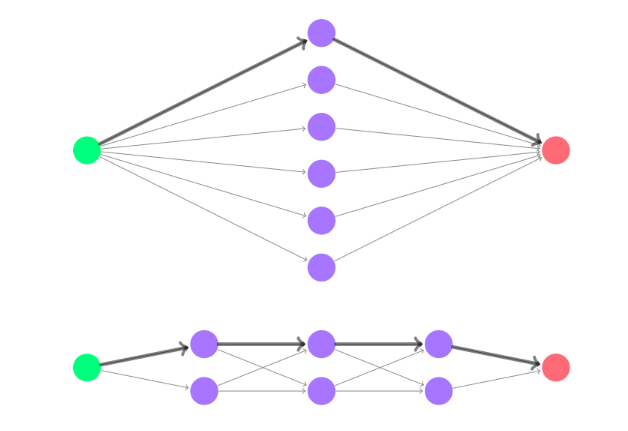
\includegraphics[scale=0.3]{images/theo5/deep-vs-narrow}
		\caption{Lợi ích của mạng học sâu}
	\end{center}
\end{figure} 

\subsubsection{Hàm kích hoạt (Activation functions)}
\begin{enumerate}
	\item \textbf{Sigmoid}
	\begin{itemize}
		\item \textit{Công thức:}
		$$\sigma(x) = \frac{1}{1 + e^{-1}}$$
		\item \textit{Ưu điểm}: hàm sigmoid có đạo hàm đẹp.
		\item \textit{Nhược điểm}: 
		\begin{itemize}
			\item Dễ gây ra các hiện tượng Vanishing / Exploding Gradient khi giá trị đầu vào có trị tuyệt đối quá lớn.
			\item Không có zero-centered, gây ảnh hưởng đến tốt độ hội tụ.
		\end{itemize}
	\end{itemize}
	\item \textbf{ReLU}
	\begin{itemize}
		\item \textit{Công thức:}
		$$ReLU(x) = max(0, x)$$
		\item \textit{Ưu điểm}: 
		\begin{itemize}
			\item Tính toán nhanh và dễ dàng do không sử dụng hàm tính lũy thừa.
			\item Tốt độ hội tụ nhanh.
		\end{itemize}
		\item \textit{Nhược điểm}: các nút có giá trị nhỏ hơn 0 qua hàm ReLU sẽ thành 0. Do đó, thông tin từ nút đấy sẽ không được truyền về cho các nút phía sau.
	\end{itemize}
	\pagebreak

	\item \textbf{Tanh}
	\begin{itemize}
		\item \textit{Công thức:}
		$$tanh(x) = \frac{e^x - e^{-x}}{e^x + e^{-x}}$$
		\item \textit{Ưu điểm}: giống với hàm sigmoid. Hàm tanh có đạo hàm đẹp. Ngoài ra, khác với sigmoid thì hàm tanh có trung tâm là 0 (zero - centered) nhờ đó mà hội tụ tốt hơn sigmoid.
		\item \textit{Nhược điểm}: Hàm tanh có 2 đầu bảo hòa giống với sigmoid. Điều này dẫn đến gradient biến mất hoặc bùng nổ.
	\end{itemize}
\end{enumerate}

\subsubsection{Bộ tối ưu (Optimizer)}
\begin{enumerate}
	\item \textbf{Gradient Descent (GD)}: 
	\begin{itemize}
		\item Tính hàm độ lỗi của toàn bộ dữ liệu huấn luyện. Sau đó tính đạo hàm và tối ưu các tham số tham chiều ngược với đạo hàm.
		\item \textit{Công thức}:
		$$x_{t+1} = x_t + \eta f'(x_t)\text{  ,trong đó $\eta$ là Learning Rate}$$ 
		\item \textit{Ưu điểm: }thuật toán dễ hiểu. Tối ưu được các thao số của mô hình sau các vòng lặp.
		\item \textit{Nhược điểm: }nghiệm tìm được phụ thuộc rất nhiều vào nghiệm khởi tạo ban đầu và learning rate. Các nghiệm khởi tạo khác nhau có thể bị rơi vào các cực trị cục bộ khác nhau và có thể không phải là nghiệm toàn cục. Learning rate quá lớn hoặc quá nhỏ sẽ làm cho quá trình hội tụ diễn ra rất lâu hoặc thậm chí không thể hội tụ. 

	\end{itemize}	
	\item \textbf{Stochastic Gradient Descent (SGD)}
	\begin{itemize}
		\item Sử dụng công thức giống với Gradient Descent. Nhưng ở mỗi epoch, ta cần tính hàm độ lỗi cho một số điểm dữ liệu và cập nhật trọng số.
		\item \textit{Ưu điểm: }đối với tập dữ liệu lớp, GD không thể tính các giá trị như hàm độ lỗi và đạo hàm một cách nhanh chóng. Tuy nhiên đối với SGD thì việc này trở nên dễ dàng.
		\item \textit{Nhược điểm: }giống với GD, SGD chưa giải quyết được vấn đề phụ thuộc và điểm trọng số khởi tạo và learning rate.
	\end{itemize}

	\item \textbf{Momentum}
	\begin{itemize}
		\item Momentum khắc phục nhược điểm của GD và SGD bằng cách thêm một lượng quán tính vào công thức tối ưu tham số. Do đó, dù có đạt đến cực tiểu, các tham số sẽ trượt lên một đoạn để có thể thoát ra khỏi cực trị địa phương hoặc là lăng ngược xuống về điểm cực trị ban đầu.
		\item \textit{Công thức}:
		\begin{align} 
			v_t = \gamma v_{t-1} + \eta f'(x)\\
			\phi = \phi - v_t
		\end{align}
		\item \textit{Ưu điểm: }thuật toán dễ hiểu. Tối ưu được các thao số của mô hình sau các vòng lặp.
		\item \textit{Nhược điểm: }nghiệm tìm được phụ thuộc rất nhiều vào nghiệm khởi tạo ban đầu và learning rate. Các nghiệm khởi tạo khác nhau có thể bị rơi vào các cực trợ cục bộ khác nhau và có thôi không phải là nghiệm toàn cục. learning rate quá lượng hoặc quá nhỏ sẽ làm cho quá trình hội tụ diễn ra rất lâu hoặc thậm chí không thể hội tụ. 
	\end{itemize}
\end{enumerate}

\subsubsection{Drop-out}
\textit{Định nghĩa:} Drop-out là kĩ thuật giúp giảm tỉ lệ overfitting của mạng nơron nhân tạo. Trong khi phương pháp Regulization trước đó đánh phạt cho trọng lượng của các tham số .Drop-out bỏ qua ngẫu nhiên một số nút trong quá trình huấn luyện theo một tỉ lệ 1-p (p được gọi là \textit{Keepting prob}). Nhờ vậy mà một nút mạng không thể phụ thuộc nhiều vào một nút mạng nào đó được (Vì không biết khi nào nút sẽ bị drop-out), từ đó mà độ phụ thuộc (trọng lượng) của các nút liên kết tới sẽ được trải đều, giúp tăng sức mạnh cho các nút mạng trong mạng. 

Hệ số p nên ở khoảng [0.2, 0.5] . Nếu p quá nhỏ thì không có tác dụng chống overfitting, tuy nhiên nếu p quá lớn thì gần như loại bỏ layer đấy và có dễ dẫn đến underfitting.

Drop-out được thực hiên trên tập validation và chia làm 2 giai đoạn:
\begin{itemize}
	\item \textbf{Training}: Với mỗi epoch, với mỗi mini-batch, ta thực hiện drop-out với tỉ lệ drop là (1-p) trên mỗi lớp ẩn.
	\item \textbf{Testing}: Ở giai đoạn testing, ta không thực hiện drop-out trên mạng. Và phải nhân một lượng p vào mỗi tham số để tránh output bị nhân lên gấp đôi.
\end{itemize}
\begin{figure}[H]
	\begin{center}
		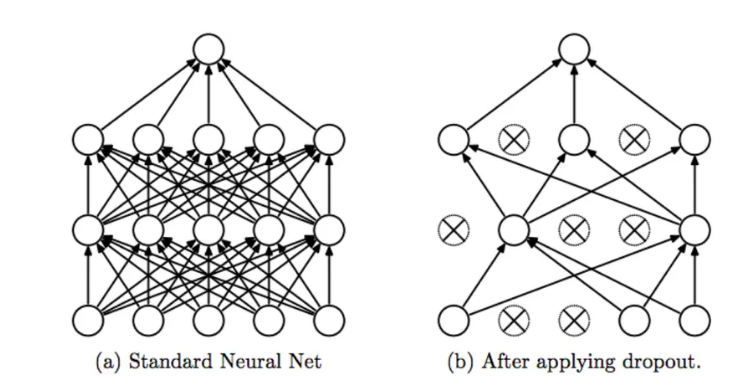
\includegraphics[scale=0.5]{images/theo5/drop-out}
		\caption{Minh họa Drop-out}
	\end{center}
\end{figure}
\pagebreak

\section{Bài tập}
\subsection{Locally Linear Embedding (LLE)}
\subsubsection{Tổng quan}

Locally Linear Embedding (LLE) là một thuật toán học không giám sát (Unsupervised Learning) dùng để giảm chiều dữ liệu phi tuyến thuộc nhóm \textit{Manifold}.

\begin{figure}[H]
	\begin{center}
		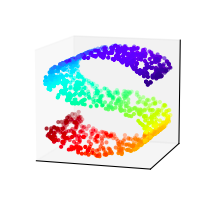
\includegraphics[scale=0.7]{images/ex1/manifold.png}
		\caption{Manifold}
	\end{center}
\end{figure}


Giải thuật LLE được nhóm tác giả \textit{Sam T. Roweis} và \textit{Lawrence K. Saul} trình bày trong bài báo "Nonlinear Dimensionality Reduction by Locally Linear Embedding" vào năm 2000.

\subsubsection{Các bài toán liên quan}
\begin{enumerate}
	\item \textbf{Face Recognition with Weighted Locally Linear Embedding}.\\ Bài toán nhận dạng khuôn mặt kết hợp với giảm chiều dữ liệu bằng thuật LLE. Qua các thực nghiệm, người ta có thể thấy rằng không gian các ảnh khuôn mặt là không gian phi tuyến có dạng đa tạp. Do đó, thuật toán LLE với khả năng giảm chiều dữ liệu phi tuyến của mình, có thể cho ra kết quả phân lớp tốt hơn so với sử dụng các giải thuật giải chiều kinh điển như PCA.
	\begin{figure}[H]
		\begin{center}
			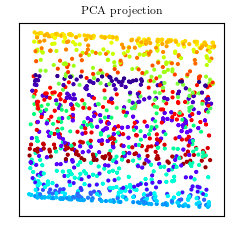
\includegraphics[scale=0.6]{images/ex1/pca.png}
			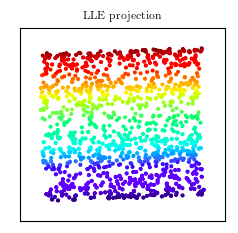
\includegraphics[scale=0.6]{images/ex1/lle.png}
			\caption{So sánh giảm chiều sử dụng PCA và LLE trên manifold}
		\end{center}
	\end{figure}
	\item \textbf{Audio Fingerprint Extraction Based on Locally LinearEmbedding for Audio Retrieval System}. 
	
	Bài toán so sánh giọng nói của một người với dữ liệu giọng nói trong database. Vấn đề của bài toán là dữ liệu âm thanh cần lưu trữ quá lớn và ảnh hưởng đến tốt độ chạy của hệ thống. Do đó, cần phải sử dụng thuật giảm chiều LLE để có thể biểu diễn âm thanh nhận dạng tốt hơn trong tập dữ liệu, giúp giảm bớt không gian lưu trữ và thời gian chạy được cải thiện.
	\begin{figure}[H]
		\begin{center}
			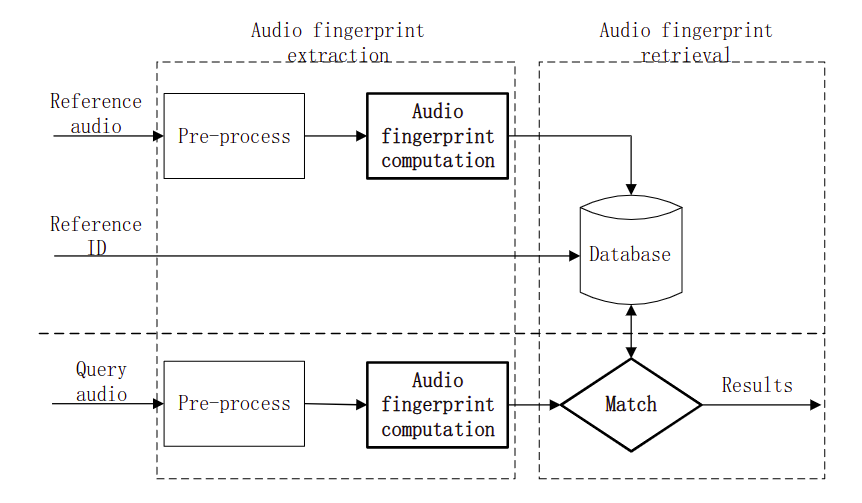
\includegraphics[scale=0.4]{images/ex1/audio-fingerprint}
			\caption{Hệ thống nhận dạng giọng nói}
		\end{center}
	\end{figure}
	\item \textbf{Supervised Locally Linear Embedding Algorithm for Hand Writting Recognition}.
	Bài toán nhận dạng chữ viết tay nói riêng và các bài toán nhận dạng mẫu nói chung thường gặp khó khăn khi chiều của dữ liệu tăng lên. Nhất là khi lượng dữ liệu trong tập không nhiều trong bài toán nhận dạng chữ viết tay. Chiều dữ liệu lớn làm cho việc nhận dạng trở nên khó khăn và tốn nhiều thời gian. Vì lý do đó, ta có thể sử dụng các thuật toán giảm chiều. 
	
	Bài toán sử dụng một một biến thể của LLE là \textit{Supervised LLE} (SLLE) để có thể áp dụng trên bài toán học có giám sát. Nhờ vào giảm chiều, sẽ tránh được các vấn đề về thiếu dữ liệu và chiều không gian lớn gây ảnh hưởng đến tính hiểu quả của giải thuật.
	\begin{figure}[H]
		\begin{center}
			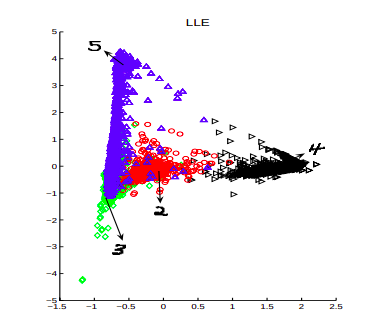
\includegraphics[scale=0.5]{images/ex1/MLLE.png}
			\caption{Hand writting Manifold}
		\end{center}
	\end{figure}
\end{enumerate}

\subsubsection{Mô tả thuật toán LLE}
\begin{enumerate}
	\item Với mỗi điểm dữ liệu p chiều, ta tìm k láng giềng gần nhất của nó.
	\item Tìm ma trận W sao cho tổng bình phương lỗi khi tái cấu trúc tuyến tính mỗi $x_i$ đạt giá trị nhỏ nhất:
	\begin{equation}
		\varepsilon(W) = \sum_{i=1}^{m}{\epsilon_i} = \sum_{i=1}^{m}{\left\|x_i - \sum_{j=1}^{n}{w_{ij}x_j}\right\|}
	\end{equation}
	\item Tìm Y sao cho tổng bình phương độ lỗi của quá trình tái cấu trúc đạt đạt giá trị nhỏ nhất:
	\begin{equation}
		\Theta(Y) = \sum_{i=1}^{n}{\left\|y_i - \sum_{j=1}^{n}{w_{ij}y_j}\right\|}
	\end{equation}
\end{enumerate}
\subsubsection{Đánh giá giải thuật}
\begin{itemize}
	\item \textbf{Ưu điểm}
	\begin{itemize}
		\item \textit{Siêu tham số}: Chỉ cần gán trước 2 siêu tham số.
		\item \textit{Tối ưu}: không liên quan đến cực tiểu cục bộ.
		\item \textit{Bảo toàn thông tin}: Thông tin không gian cục bộ trong không gian nhiều chiều được bảo toàn trong không gian con.
		\item \textit{Độ phức tạp:} LLE được cài đặt trong bộ thư viện scikit-learn là: $$\mathbf{O}[D log(k) m log(m)] + \mathbf{O}[Dmk^3] + \mathbf{0}[dm^2]$$
		Có thể thấy thuật toán chạy trong thời gian đa thức và phụ thuộc mạnh mẽ vào số lượng láng giếng k.
		\item \textit{Thư viện hỗ trợ:} Trong python, Locally Linear Embedding được cài đặt trong thư viện scikit-learn (sklearn.manifold.LocaLinearEmbedding).
	\end{itemize}
	\item \textbf{Nhược điểm}
	\begin{itemize}
		\item Nếu mật độ các mẫu không dày, hoặc việc lấy mẫu không đều, có thể tạo ra các manifold không đồng nhất, hay nói cách khác có nhiều manifold hình thành nên bộ dữ liệu, từ đó gây ra hiểu nhầm trong lúc chạy thuật.
		\item LLE rất nhạy cảm với nhiễu, với một lượng nhiễu nhỏ cũng có thể dẫn đên lỗi khi tạo embedding. 
		\item Không đảm bảo 2 điểm khác nhau trong không gian nhiều chiều sẽ khác nhau trong không gian giảm chiều. 
		\item Phụ thuộc nhiều vào 2 siêu tham số k và d. Việc chọn 2 siêu tham số không tốt có thể dẫn đến thuật toán không cho kết quả tốt.
		\item Chỉ dùng cho các bài toán học không giám sát. (Sau đó đã có các biến thể SLLE để giải quyết các bài toán học có giám sát).
	\end{itemize}
\end{itemize}
\subsection{ArcFace}
\subsubsection{Bài toán}
Các mạng học sâu giải quyết các bài toán phân lớp gương mặt thường sử dụng hàm lỗi softmax để tính xác suất của một ảnh gương mặt thuộc về đối tượng nào. Nhưng khi số lượng ảnh trong cơ sở dữ liệu tăng đáng kể ngày nay, hàm softmax khó có thể phân biệt các điểm dữ liệu ở gần biên của 2 đối tượng khác nhau.\\
ArcFace sử dụng hàm lỗi Additive Angular Margin với mục tiêu gom các ảnh cùng một đối tượng lại gần nhau và các cụm đối tượng khác nhau sẽ xa nhau trong không gian latent space. Từ đó, tăng được độ hiệu quả trong các bài toán nhận dạng mặt người.\\
ArcFace là một giải pháp được phát triển bởi InsightFace - một dữ án open source cung cấp thư viện các thuật toán nhận dạng gương mặt 2D và 3D. Được trình bài trong bài báo "Additive Angular Margin Loss for Deep Face Recognition" được đăng tải trên \textit{arxiv.org} vào 23/01/2018.\\
Đối tượng tiềm năng cho giải pháp này là các hệ thống an ninh của chính phủ, khi cần quản lý rất nhiêu các đối tượng khác nhau. Hơn thế, đôi khi có các đối tượng có gương mặt khá giống nhau khiến cho khoảng cách giữa chúng trong latent space khá gần nhau dẫn đến khó nhận dạng.\\
Ta có thể tìm thấy các thông tin về ArcFace như demo minh họa, bài báo khoa học, mã nguồn tại trang \url{https://insightface.ai/arcface}
\subsubsection{Tính năng chủ đạo}
Tính năng chủ đạo của giải pháp là gom các embedding của cùng một đối tượng lại gần nhau và tách rời các cụm đối tượng ra xa nhau. Cụ thể thuật toán hoạt đông như sau:

\textit{ArcFace} đã đưa ra ý tưởng sử dụng các vector tham số làm tâm của các lớp và từ đó tối ưu "khoảng cách" giữa các điểm dữ liệu đến tâm của nó. Ta có thể hình dung được rõ hơn qua công thức sau đây:
\begin{equation}
    W_{j}^{T}x_i = \|W_j\|\cdot\|x_i\|\cos{\theta_j}
\end{equation}

Với $W_j$ là vector tham số tương ứng với lớp thứ j, $x_i$ là điểm dữ liệu và $\theta_j$ là giữa giữa $W_j$ và $x_i$.  

Ta thực hiện chuẩn hóa ($L_2$ normalisation) lên các vector $W_j$ và $x_i$. Và nhân các $x_i$ với 1 lượng s. Bằng cách chuẩn hoán như trên, ta sẽ có $\|W_j\|=1$ và $\|x_i\|=s$, nhờ đó mà dự đoán khi phân lớp chỉ phụ thuộc vào $\theta_j$. Công thức (7) được đổi thành:  
\begin{equation}
L_2=-\frac{1}{N}\sum_{i=1}^{N}{\log{\frac{e^{s\cos{\theta_{y_i}}}}{e^{s\cos{\theta_{y_i}}} + \sum_{j=1,j\neq y_i}^{N}{e^{s\cos{\theta_{j}}}}}}}
\end{equation}

Từ (10), ta có thể hình dung ra các embedding sẽ tập trung xung quanh các tâm của lớp và phân bố trên 1 mặt siêu cầu (\textit{hypersphere}). Sau đó, ta cộng một siêu tham số \textit{m (Additive Angular Margin)} vào góc giữa $x_i$ và $W_j$ để có thể tối ưu tốt hơn các khoảng cách giữa các embedding. Minh hoạ bằng hình bên dưới, ta thấy khi sử dụng hàm \textit{Softmax loss} để phân lớp, đường ranh giới giữa các lớp rất mờ, khiến cho việc phân lớp cho các điểm gần ranh giới này dễ xảy ra sai sót. Còn đối với \textit{Additive angular margin loss} bằng các sử dụng margin để ngăn cách giữa các lớp, Các điểm dữ liệu co cụm lại gần tâm của nó để  lại một khoảng cách xa giữa các lớp từ đó giúp quá trình phân lớp ít lỗi hơn.

\begin{figure}[H]
    \begin{center}
        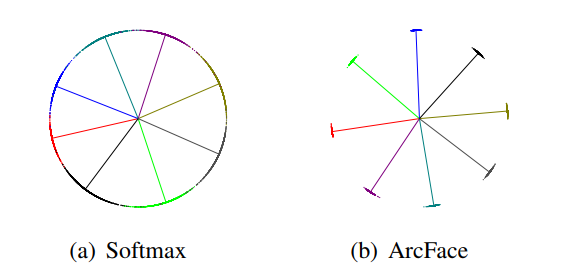
\includegraphics[scale=0.5]{images/ex2/softmax-vs-arcface}
        \caption{So sánh giữa softmax và afcface}
    \end{center}
\end{figure}

\textbf{Ưu điểm}
\begin{itemize}
	\item Độ phức tạp thấp, hiệu suất cao, lập trình dễ dàng.
	\item Có độ hội tụ tốt trên các tập dữ liệu khác nhau mà không cần kết hợp thêm hàm độ lỗi nào khác.
\end{itemize}
\textbf{Nhược điểm}
\begin{itemize}
	\item Khi số lượng các lớp tăng lên thì ma trận W cũng sẽ tăng lên đáng kể.
	\item Sử dụng hàm arccos khi chi phí tính toán chưa tối ưu.
\end{itemize}

\textbf{Tiềm năng phát triển}: \textit{ArcFace} đang mở ra các hướng đi mới trong việc giaỉ quyết các bài toán nhận dạng khuôn mặt với số đối tượng cần nhận dạng quá nhiều. Có thể thấy sự phát triển của giải pháp này trong quá khứ từ \textit{SphereFace} đến \textit{CosFace} và giờ là \textit{ArcFace} đang là state-of-the-art trong các bài toán nhận dang khuôn mặt. Và trong tương lai, hướng giải quyết này sẽ còn có khả năng phát triển để có thể giúp các tổ chức chính phủ quản lý người dân, thắt chặt an ninh và truy vết, bắt giữ các phần tử nguy hiểm trong xã hội nhanh chóng.

Có thể có cái nhìn tổng quát hơn về khác biệt của các độ lỗi bằng hình bên dưới, có thể thấy các phương pháp \textit{SphereFace} và \textit{CosFace} có các đường biên quyết định (\textit{decision boundary}) có dạng phi tuyến, trong khi \textit{ArcFace} lại cho kết quả tuyến tính giúp phân lớp dễ dàng hơn.  

\begin{figure}[H]
    \begin{center}
        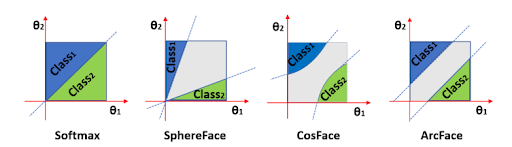
\includegraphics[scale=0.7]{images/ex2/loss-cmp}
        \caption{So sánh giữa giữa các độ lỗi}
    \end{center}
\end{figure}



\subsection{Đa dạng trong giải thuật học máy}
\subsubsection{Bài toán}
Bài toán \textit{Speech Recognition} với đầu vào là một đoạn audio được thu âm và đầu ra là đoạn văn bản chính xác câu của người nói.
\subsubsection{Giải pháp sử dụng CNN}
\begin{itemize}
	\item Giải pháp sử dụng mạng CNN kết hợp với HMM.
	\item \textbf{Tư tưởng chủ đạo: } Sử dụng mạng CNN để học xác suất hậu nghiệm của đoạn âm thanh, từ đó HMM sử dụng output của CNN để dự đoán các likelihood của từng frame âm thanh. Các likelihood này sẽ được Viterbi decoder tạo ra đoạn văn bản hoàn chỉnh.
	\item \textbf{Các bước chính: }
	\begin{itemize}
		\item \textbf{Bước 1: }Đoạn âm thanh ở miền thời gian được chuyển thành melspectrogram. 
		\item \textbf{Bước 2: }Melspectrogram sau đó được được đưa vào mạng CNN và qua một lớp softmax để output được xác suất hậu nghiệm.
		\item \textbf{Bước 3: }Xác suất hậu nghiệm này sẽ được sử dụng để dự đoán các likelihood của từng frame.
		\item \textbf{Bước 4: }Các likelihood sẽ được bộ giải mã Viterbi chuyển thành đoạn văn bản hoàn chỉnh.
		\item \textbf{Bước 5: }So sánh đoạn văn bản dự đoán và đoạn văn bản đúng để học các tham số trong mô hình.
	\end{itemize}
	\item \textbf{Bài báo khoa học: }
	\href{https://www.microsoft.com/en-us/research/wp-content/uploads/2016/02/CNN_ASLPTrans2-14.pdf}{Tại đây}.
	\item \textbf{Ưu điểm: } 
	\begin{itemize}
		\item Số ượng tham số ít hơn so với sử dụng DNN. Nhờ sử dụng weight sharing.
		\item Có thể học được các đặc trưng phân cấp của đoạn âm thanh.
	\end{itemize}
	\item \textbf{Nhược điểm: }
	\begin{itemize}
		\item Cần sử dụng nhiều dữ liệu, trong khi để thu thập được một lượng lớn âm thanh và transcript cho từng đoạn âm thanh đôi khi gặp nhiều khó khăn.
		\item Do sử dụng nhiều dữ liệu, nên tài nguyên tính toán cũng tăng theo đáng kể dẫn đến cần các tài nguyên phân cứng mạnh để có thể chạy các mô hình CNN. 
	\end{itemize}
\end{itemize}
\subsubsection{Giải pháp sử dụng RNN}
\begin{itemize}
	\item Giải pháp sử dụng mạng Bidirectional LSTM kết hợp với CTC loss.
	\item \textbf{Tư tưởng chủ đạo: }Với mỗi timestep sẽ sẽ dự đoán xem frame đấy sẽ là kí tự nào (các khả năng sẽ gồm tất cả các ký tự và một ký tự rỗng). Từ đoạn văn bản thô đấy, ta hình thành đoạn văn bản kết quả theo quy tắt: các ký tự (Không bao gồm ký tự rỗng) giống nhau liên tiếp sẽ gom lại thành một ký tự.\\
	\\
	\textit{Ví dụ:} ký tự rỗng được biểu diễn bằng "-"
	\begin{itemize}
		\item "hhh---e-ll---lll---oo--- ---wwww-oooo---r--ll---dd" $\rightarrow$ "hello world"
		\item "SS--ooo-n- ---dd--e---pppp--- -----t-rr--aaa---iiiiiiiiiii" $\rightarrow$ "Son dep trai"
	\end{itemize}
	\item \textbf{Các bước chính:}
	\begin{itemize}
		\item \textbf{Bước 1: }Đoạn âm thạnh ở miền thời gian được chuyển thành melspectrogram. 
		\item \textbf{Bước 2: }Từng frame $x_t$ của melspectrogram sẽ được input vào BLTSM và output ra vector $y_t$ với ý nghĩa là độ thuộc của của $x_t$ với các ký tự trong tập dự đoán. $y_t$ sẽ được đưa vào một lớp softmax để thu được phân bố xác suất của ký tự thứ k tại frame thứ t ($Pr(k\vert t)$)
		\item \textbf{Bước 3: }Sử dụng Gradient Descent để học các tham số của CTC và BLSTM.
	\end{itemize}
	\item \textbf{Bài báo khoa học: } \href{https://ieeexplore.ieee.org/document/6638947}{Tại đây}
	\item \textbf{Ưu điểm: }do là mô hình theo kiến trúc end-to-end nên sẽ không cần quan tâm đến các giai đoạn như tiền xử lý hay rút trích đặt trưng của dữ liệu đầu vào. Đoạn âm thanh sẽ được chuyển trực tiếp thành văn bản thông qua mô hình. 
	\item \textbf{Nhược điểm: }Mô hình sử dụng chiến thuật tham lam khi phân bố xác suất ở mỗi timestep chỉ phụ thuộc vào kí tự trước đó. Để giải quyết vấn đề này. Trong bài báo trên, nhóm tác giả có đề xuất sử dụng RNN Transducer để có độ phân bố của ký tự dự đoán so với tất cả các ký tự trước đó đã được dự đoán. Sau đó sử dụng Beam Search để decode ra ký tự dự đoán.

\end{itemize}
\pagebreak

\section{Tài liệu tham khảo}
\begin{itemize}
    \item Slide bài giảng trên trang môn học.
    \item \href{https://www.researchgate.net/publication/283539781_Adjacent_evaluation_of_local_binary_pattern_for_texture_classification}{Adjacent Evaluation LPB}
    \item \href{https://machinelearningcoban.com/2017/06/15/pca/}{Bài 27: Principal Component Analysis (machinelearningcoban)}
    \item \href{https://machinelearningcoban.com/2017/06/30/lda/}{Bài 29: Linear Discriminant Analysis(machinelearningcoban)}
    \item \href{https://machinelearningcoban.com/2017/04/09/smv/}{Bài 19: Support Vector Machine (machinelearningcoban)}
    \item \href{https://machinelearningcoban.com/2017/04/22/kernelsmv/}{Bài 21: Kernel Support Vector Machine (machinelearningcoban)}
    \item \href{https://aicurious.io/posts/2019-09-23-cac-ham-kich-hoat-activation-function-trong-neural-networks/}{Hàm kích hoạt (activate function)}
    \item \href{https://viblo.asia/p/optimizer-hieu-sau-ve-cac-thuat-toan-toi-uu-gdsgdadam-Qbq5QQ9E5D8}{Tối ưu (Optimizer)}
    \item \href{https://www.phamduytung.com/blog/2019-05-05-deep-learning-dropout/}{Kĩ thuật Drop-out}
    \item \href{https://qastack.vn/stats/82037/explain-steps-of-lle-local-linear-embedding-algorithm}{Thuật toán LLE}
    \item \href{https://www.astroml.org/book_figures/chapter7/fig_S_manifold_PCA.html}{Comparison of PCA and Manifold Learning}
    \item \href{https://ieeexplore.ieee.org/document/1443143}{Face recognition with weighted locally linear embedding}
    \item \href{https://www.researchgate.net/publication/344815452_Audio_Fingerprint_Extraction_Based_on_Locally_Linear_Embedding_for_Audio_Retrieval_System}{Audio Fingerprint Extraction Based on Locally Linear Embedding for Audio Retrieval System}
    \item \href{https://www.researchgate.net/publication/221258597_Supervised_Locally_Linear_Embedding_Algorithm_for_Pattern_Recognition}{Supervised Locally Linear Embedding Algorithm for Pattern Recognition}
    \item \href{https://arxiv.org/abs/1801.07698}{ArcFace: Additive Angular Margin Loss for Deep Face Recognition}
    \item \href{https://www.youtube.com/watch?v=H1qEp_czI1I&t=51s}{ArcFace explained video}
    \item \href{https://github.com/peteryuX/arcface-tf2}{ArcFace for face verification}
\end{itemize}


\end{document}
